\documentclass[output=paper]{../langscibook}
\ChapterDOI{10.5281/zenodo.4449778}
\author{Julia Barnes\affiliation{Mondragon University}\orcid{}\lastand Margareta Almgren\affiliation{ University of the Basque Country}}
\title{Training teachers for the challenges of multilingual education}
\abstract{This chapter focuses on how trainee teachers are prepared to face the linguistic complexity they will encounter in classrooms in the Basque Autonomous Community (henceforth BAC) in Spain. Although Spanish is the home language for most children in the BAC, the overwhelming majority of parents choose Basque as language of instruction at pre-school and primary levels (\citealt{BasqueGovernment2018}) independently of the language spoken at home, which means that Basque is mainly acquired through immersion programmes. The teacher training programme at 
Mondragon University aims at providing future pre-school and primary teachers with solid knowledge on language acquisition in bi/multilingual contexts. These future teachers are also made familiar with instruments for measuring children’s language development and, furthermore,  they carry out a team-work project to be presented in English, containing data on children’s linguistic picture as well as reflections on their own linguistic skills and the utility of knowledge acquired for their future in multilingual education.}
\IfFileExists{../localcommands.tex}{
  \addbibresource{../localbibliography.bib}
  % add all extra packages you need to load to this file

\usepackage{tabularx,multicol}
\usepackage{url}
\urlstyle{same}

\usepackage{enumitem}

\usepackage{pifont}

\usepackage{listings}
\lstset{basicstyle=\ttfamily,tabsize=2,breaklines=true}

\usepackage{./langsci-optional}
\usepackage{./langsci-lgr}
\usepackage{./langsci-gb4e}

\usepackage{langsci-plots} 

\makeatletter
\let\pgfmathModX=\pgfmathMod@
\usepackage{pgfplots,pgfplotstable}%
\let\pgfmathMod@=\pgfmathModX
\makeatother

\usepackage{siunitx}
\sisetup{output-decimal-marker={.},detect-weight=true, detect-family=true, detect-all, input-symbols={\%}, free-standing-units,table-align-text-pre=false,group-digits=false,detect-inline-weight=math}
\DeclareSIUnit[number-unit-product={}]{\percent}{\%}
\makeatletter \def\new@fontshape{} \makeatother
\robustify\bfseries % For detect weight to work

\usepackage{todonotes}

  \newcommand*{\orcid}{}

\renewcommand{\lsChapterFooterSize}{\footnotesize}

\makeatletter
\let\thetitle\@title
\let\theauthor\@author
\makeatother

\newcommand{\togglepaper}[1][0]{
%   \bibliography{../localbibliography}
  \papernote{\scriptsize\normalfont
    \theauthor.
    \thetitle.
    To appear in:
    Jorge Pinto \& Nélia Alexandre (eds.),
    Multilingualism and third language acquisition: Learning and teaching trends.
    Berlin: Language Science Press. [preliminary page numbering]
    }
  \pagenumbering{roman}
  \setcounter{chapter}{#1}
  \addtocounter{chapter}{-1}
}


 
  %% hyphenation points for line breaks
%% Normally, automatic hyphenation in LaTeX is very good
%% If a word is mis-hyphenated, add it to this file
%%
%% add information to TeX file before \begin{document} with:
%% %% hyphenation points for line breaks
%% Normally, automatic hyphenation in LaTeX is very good
%% If a word is mis-hyphenated, add it to this file
%%
%% add information to TeX file before \begin{document} with:
%% %% hyphenation points for line breaks
%% Normally, automatic hyphenation in LaTeX is very good
%% If a word is mis-hyphenated, add it to this file
%%
%% add information to TeX file before \begin{document} with:
%% \include{localhyphenation}
\hyphenation{
affri-ca-te
affri-ca-tes
au-ton-o-mous
Cha-basse
Din-ger-fel-der
plu-ri-lin-gual
Ya-na-pra-sart
Mi-ri-ci
Ström-quist
}

\hyphenation{
affri-ca-te
affri-ca-tes
au-ton-o-mous
Cha-basse
Din-ger-fel-der
plu-ri-lin-gual
Ya-na-pra-sart
Mi-ri-ci
Ström-quist
}

\hyphenation{
affri-ca-te
affri-ca-tes
au-ton-o-mous
Cha-basse
Din-ger-fel-der
plu-ri-lin-gual
Ya-na-pra-sart
Mi-ri-ci
Ström-quist
}
 
  \togglepaper[1]%%chapternumber
}{}

\begin{document}
\maketitle 
%\shorttitlerunninghead{}%%use this for an abridged title in the page headers



 \section{Introduction}


Today’s globalised world is becoming increasingly aware of the fact that most of its inhabitants are no longer monolinguals. Traditionally, a much-discussed issue in childhood bilingualism has been that of mixing and separation of codes \citep{Meisel2001} or crosslinguistic influence \citep{Lanza1998,MullerHulk2001}, and much effort was given to discussing the theme of balanced or unbalanced bilingualism \citep{DeHouwer2009}. Recently the perspective has been changing. Rather than aiming at, and evaluating, native-like competence in a bi/multilingual person’s languages, the new approach takes into account each individual’s total language repertoire from a holistic and dynamic perspective. This “multi-competence” perspective \citep{Aronin2016} proves useful when analysing the wide variety of situations in multilingual communities. In such contexts it is paramount to view “someone who knows two or more languages  [to be] a different person from a monolingual, and so needs to be looked at in their own right rather than as a deficient monolingual” (\citealt{Cook2013}, p.3768). As a consequence, the focus of interest is changing from monolingualism/bilingualism to multilingualism, both from the point of view of multilingual individuals and multilingual societies. 

It is also important to take into account the difference made between multilingualism as a social phenomenon and multilinguality, as referred to individuals. Although in many cases multilingual individuals live in multilingual communities, this is not always the case. It may well be that in a bi/multilingual community, as the case referred to in the present article, many speakers are monolingual. On the contrary bi/multilingual speakers may also live in monolingual communities, as in the case of a German-dominant child exposed to French from one parent \citep{Meisel2008}.

Today’s multilingual speakers are also in many cases L2 speakers of some of their languages, and therefore the concept of \emph{dominant language constellation}, DLC, \citep{Aronin2016} becomes extremely pertinent when analysing both social and individual use of languages. DLC refers to one person’s or one community’s most dominant languages and their domain of use and fits very well into the situation we will deal with. We will explore how students of the Basque Country become aware of their own multilingual skills by examining young children’s language development, and how they begin to understand the different DLCs they will encounter in their professional future as infant teachers.


\section{The sociolinguistic situation of the Basque Country}
\largerpage

Basque, a non-Indo-European language of unknown origin, is currently spoken by approximately 34\% of the population of the Basque Autonomous Country (henceforth BAC) in northern Spain and understood by another 20\% (\citealt{BasqueGovernment2017}). Since Basque became co-official with Spanish in the BAC in 1979 and compulsory in education in 1982, its weight in primary education has steadily grown. It was introduced offering three educational models for parents to choose between: In the A model, education is provided in Spanish and Basque is a subject matter for 3 or 4 hours a week. In the B model, both Spanish and Basque are languages of instruction. In the D model, (C is not used in Basque) Basque is the language of instruction and Spanish is a subject matter for 3 or 4 hours a week.

\largerpage
Initially, the possibility of using Basque in education at the same level as Spanish was seen with certain incredulity, in particular by the rural Basque-speaking population by whom Spanish was perceived as the prestige language. In 1985 around 16\% of primary children were schooled in Basque, and 8\% in the bilingual model B. During the following decades, the positive results obtained in education in Basque, both in academic aspects and as to language skills in Basque and Spanish, slowly convinced the majority of the population of the benefits of education in Basque \citep{Cenoz2009}. In 2018, the D model was chosen by 78.9\% of the families and the B model by another 17.3\% \citep{BasqueGovernment2018}. Taking into account that Basque is L1 only for 23\% of the children, it is evident that schooling in Basque means full or partial immersion for many children and is producing a generational shift in new speakers of the Basque language as a result of effective education policy in a situation of sociolinguistic complexity (\citealt{AmorrortuEtAl2009};  \citealt{OrtegaEtAl2015}).

 In order to respond to the increasing demand for instruction in Basque, an intense effort had to be made in order to prepare teachers for this task. On the one hand, Basque-speaking teachers in the Spanish educational system before 1982 were usually not literate in Basque. They were speakers of different oral varieties of Basque but had no instruction in the standardised written language “euskara batua”, established in 1968. On the other hand, most teachers were not Basque speakers and had to start learning the language from scratch. A considerable effort has been made both by these teachers and by the department of education of the Basque government in terms of providing paid training. Due to this effort, the number of teachers able to teach (in) Basque has increased from around 5\% in 1978 to over 90\% in 2016 (\citealt{BasqueGovernment2017}).

However, acquiring knowledge of, and even fluency in, a language is not equivalent to knowing how to teach it. And even if teachers are prepared to teach Basque as L2, or even to teach in Basque as L1, the situations they will meet in classrooms are complex; children whose home language is Basque are usually mixed with children who have had some contact with Basque outside school, or those who have had no contact whatsoever with Basque. In addition, the sociolinguistic context spans over environments where Basque is the principle language used in the community, where Basque and Spanish are used alongside each other, and environments where no Basque at all is spoken. These are factors which show that specific training is needed.


\subsection{Infant and pre-primary school teacher training at Mondragon University}


In the following lines, we will focus on how trainee teachers are prepared to confront the linguistic complexity they will inevitably encounter in classrooms across the BAC. The present approach to teacher training was initiated in 2009, as part of the Bologna process, but here we will limit our discussion to data from the 2017--2018 cohort.  

As pointed out, although Spanish is the home language for most children in the BAC, the overwhelming majority of parents choose Basque as language of instruction at pre-school and primary levels independently of the home language, which means that Basque is mainly acquired through immersion programmes. In addition to Basque and Spanish, English is often introduced as a third language by the early age of 4 and students are expected to reach B1 competence by the end of post-secondary education \citep{Lasagabaster2000}. Some children are also exposed to other languages at home \citep{Barnes2006}. All these children are schooled together in mixed groups, so it can be concluded that as a result, multilingualism is becoming the norm in the BAC \citep{Cenoz2009}.

If a school wishes to teach 3 or 4 languages it is clearly necessary to plan the progressive introduction of each one to fulfil the linguistic objectives set down by the Basque department of education. Consequently, all future teachers from any specialism, who are themselves Basque-Spanish bilinguals (many of them L2 speakers of Basque), will need enhanced awareness of psycholinguistic and sociolinguistic requirements for educating Basque L1 children alongside Spanish L1 children in Basque immersion, together with pupils from other linguistic backgrounds, particularly in infant classrooms where language is still developing. This raises some issues from a training perpective.  How aware are future teachers of young bilinguals of the linguistic complexity in their classrooms? Do they realise the variety of situations of input their pupils are exposed to? Are they familiar with instruments with which evidence of language development and sociolinguistic development can be measured? To what extent are Basque L1 and L2 trainees (who are not language teaching specialists) able to reflect upon (in writing) and act upon (in teaching) good practice in classrooms?


\subsection{Teaching model and methodology}


To better understand this, we will analyse features such as the linguistic competence and attitudes towards language learning of Basque-Spanish bilingual trainee infant and pre-primary (0--6 years) teachers who annually complete a six credit module through the medium of English in years 1, 2, and 4 of their education degree, in undergraduate training in infant education at Mondragon University in the Basque Country. These students are not training to be English teachers, but we should point out that the modules are in English for two main reasons, namely to develop their personal multilingual skills (they have received compulsory English tuition for 14 years within the education system) and to give them the skills and confidence necessary to use their third language if required to do so in their future teaching activity. English is increasingly present in Basque infant education in different spaces across the curriculum, and novice teachers are often considered able to carry out activities in English.

The teaching modules within the Mondragon University curriculum which are delivered in English as a third language cover:

\begin{itemize}
\item Education and good practice in Europe and the global world (first year six credit module), 
\item Learning and teaching of second languages in multilingual contexts (second year six credit module) 
\item Lifeplace learning (fourth year six credit module) 
\end{itemize}

This paper reports on the second year module, \emph{learning and teaching of second languages in multilingual contexts}, by the end of which students are required to have the initial theoretical knowledge to understand the principles behind the acquisition of first and second languages in monolingual, bilingual and multilingual contexts. The module includes basic concepts in relation to age factor in the acquisition of languages and of interaction and inter-language. To this effect, students are provided with literature on language acquisition (\citealt{Genesee1994}; \citealt{LightbownSpada2013}; \citealt{Palenham2004}) in order to acquire theoretical knowledge to be applied in the projects they will carry out. They are also made aware of affective and emotional states that may influence language acquisition (\citealt{Barnes2006}; \citealt{DeHouwer2009,DeHouwer2009b}; \citealt{Dewaele2013}. The module closes with a contrasting practical focus on incorporating classroom and linguistic strategies appropriate to what has been learned, through the design and peer-teaching of a short activity. This work is further developed in a module in the third year of the degree, where the topics are reviewed and developed through the medium of Basque.

The principle aim of the second year module of our interest here is to identify difficulties in communication and learning when the language of instruction is new to the learner, to show empathy to children in immersion contexts and to enable students to make use of strategies to aid learning, particularly language learning, in such contexts. Additionally, students develop their own language skills, through reflection on their own language acquisition process(es) and through working through the medium of their third language, English. Academic reading skills are developed through designated chapters relating to language acquisition from \citet{Palenham2004}.

The module is divided into four units, which feed into two practical assessed Projects.

Project 1, \emph{One child's linguistic picture}, covers the first two units of the module:

\begin{enumerate}
\item Learning about affective factors in language learning: students reflect on the experience of a “well-taught” and a “badly taught” language lesson in a new language (provided by Erasmus students) and extend this to how children may feel in immersion classrooms.
\item Linguistics: the basic principles behind the acquisition of first and second languages in monolingual, bilingual and multilingual formal and informal contexts during childhood 
\end{enumerate}

The project consists of a small-scale research study in which students are required to collect a sample of child language to examine to identify evidence of the multiple processes that take place during language acquisition and takes place over a period of two months.

Project 2 covers the second two units of the module: 

\begin{enumerate}[start=3]
\item Immersion and integrated curriculum in infant school. 
\item Good practice in infant-junior language teaching
\end{enumerate}

Students create, peer-teach and justify an activity appropriate for a classroom context specified by the tutor. This activity should be governed by best practice and the requirements for infant language development as described in the curricular guidelines of the Basque education department. Project 2 also involves the design and preparation of a mini-conference. Student groups prepare poster presentations and accompanying handouts in which they display and explain to each other different aspects of methodology and materials appropriate for language learning in early years education. This project lasts approximately one month.

The focus of the present study is the Project 1, titled \emph{one child's linguistic picture} (henceforth OCLP), which is central to the whole module and will be addressed in more detail in the following sections.


\section{\emph{One child's linguistic picture} (OCLP) project}
\subsection{Instruments for measuring child language development}

As shown above, during their second year studies through the medium of English, teacher trainees have reflected on their own learning process as bilinguals, as learners of a foreign language (English) and their feelings when confronted with a language which is completely new to them. They have also learned about various aspects of language acquisition and bi/multilingualism. Subsequently, and in order to consolidate this learning, students take part in a multilingual small-scale research project, the OCLP, about the linguistic development of 4-year-old children in Basque and Spanish. To this effect, they are made familiar with instruments such as the Peabody picture vocabulary test \citep{DunnEtAl1986}, the MacArthur-Bates CDI III \citep{Dale2007}, and narrative elicitation tools. These tools will, in conjunction, provide a broad assessment of the chosen child's understanding in both languages (Peabody test), production in both languages (\emph{Bird story}) and of parental report on the child's understanding and production in both languages (KGNZ). The goal of this data collection, rather than to undertake a scientific study on children's receptive and productive skills, is for trainee teachers to become aware of some aspects of child language acquisition. 

The Peabody vocabulary test is a widely-known instrument used to measure receptive vocabulary ability, often applied with diagnostic purposes by speech therapists. First designed for testing the understanding of standard American English, its use has been extended to other languages, since it is based on linking a word the examiner says to one of four pictures. Consequently, it can be used on one and the same subject both for Basque and for Spanish for comparative purposes. It was adapted into Basque for the purposes of the OCLP project, but not validated. Since the purpose was to obtain an impression of the child's understanding, students were made aware of this and data cannot be considered scientifically reliable.

The MacArthur-Bates communicative development inventory (CDI) questionnaires are based on parental reports on their children’s receptive (CDI I) and productive (CDI I, II and III) vocabulary. It was also first developed for American English, but has subsequently been adapted to nearly 100 languages throughout the world.\footnote{\url{http://mb-cdi.stanford.edu/}} These questionnaires were originally developed for use by paediatricians and speech therapists, but they have since been widely used in research on child language (\citealt{FensonEtAl1994}; \citealt{BatesEtAl1995}; \citealt{Kern2007}; \citealt{EricssonEtAl2012}). The CDI questionnaires have also been used to reflect language development in bilingual children in different language communities. For this purpose, monolingual questionnaires -- one for each language -- have been used in most cases, such as Galician-Spanish \citep{Perez-Pereira2008}, Basque-Spanish \citep{EzeizabarrenaEtAl2018} and Spanish-English \citep{CoreEtAl2013}. In a few cases, such as Irish-English (\citealt{OTooleHickey2016}) and Maltese-English \citep{GattEtAl2014} specific bilingual questionnaires are available.

The CDI I for ages 8--15 months and the CDI II for ages 16--30 months have also been adapted into Basque as KGNZ I and II by \citet{BarrenaEtAl2008} and into Spanish as iLG (\citealt{Lopez_OrnatEtAl2003}). A further version for children up to 37 months of age known as CDI III was developed for American English and adapted to Basque as KGNZ III \citep{GarciaEtAl2014}. The Basque KGNZ versions have proved to be valid up to age 40 months. The CDI includes calculating mean length of utterance, based on the 3 longest sentences the child has produced, as reported by parents on the questionnaire. The MLU may be calculated on the average number of words, MLUw, or on the average number of morphemes, MLUm. Taking into account that in the Basque Country children are often exposed to both Basque and Spanish, the KGNZ also contains a section where parents are asked to estimate input in Basque, or Basque and Spanish, in relation to the number of hours a day and days a week. This is of interest because sole exposure to Basque usually takes place in the family and at early ages with incresing social exposure to Spanish over time.  When comparing monolingual Basque and bilingual Basque-Spanish development the data collected with the KGNZ questionnaires reveal that if input in Basque is above 60\% no significant differences appear in the productions of monolingual and bilingual subjects, prior to the age of 24 months. However, after this age amount of input is revealed to be decisive in rate of development \citep{EzeizabarrenaEtAl2013}.

So far no standardised Spanish version of the CDI III is available. For the purposes of the present OCLP project a translated version of the Basque KGNZ III was used. Evidently, the data collected should be interpreted with caution, but it should be born in mind that the main purpose was not, in this case, to collect statistically valid data on the children but to make students acquainted with different instruments and enable them to interpret their findings.

The wordless picture story \emph{Frog, where are you?} \citep{Mayer1969} has been used in numerous studies on children’s narrative skills \citep{BermanSlobin1994,StromquistVerhoeven2004}. During the early years of the OCLP project it was used by the second year students at Mondragon University, but feedback suggested that children nowadays, accustomed to colourful stories in books and digital resources, seemed no longer to be attracted by the black-and-white Frog story.

During the last two academic years of our students’ training courses, the Frog story has been replaced by the \emph{Bird story} from the COST project \citep{COST2012}. The images (in their coloured version) are unfolded in sequential order to the children, who are asked to tell the story. The trainee teachers are strongly advised against allowing the test to be a question-and-answer session as the objective is to collect evidence of the child's narrative production in each language, rather than of the child's interactive skills with an interlocutor. However, the students are also encouraged to be aware of the child's anxiety, and proceed accordingly.

% \begin{figure}
%   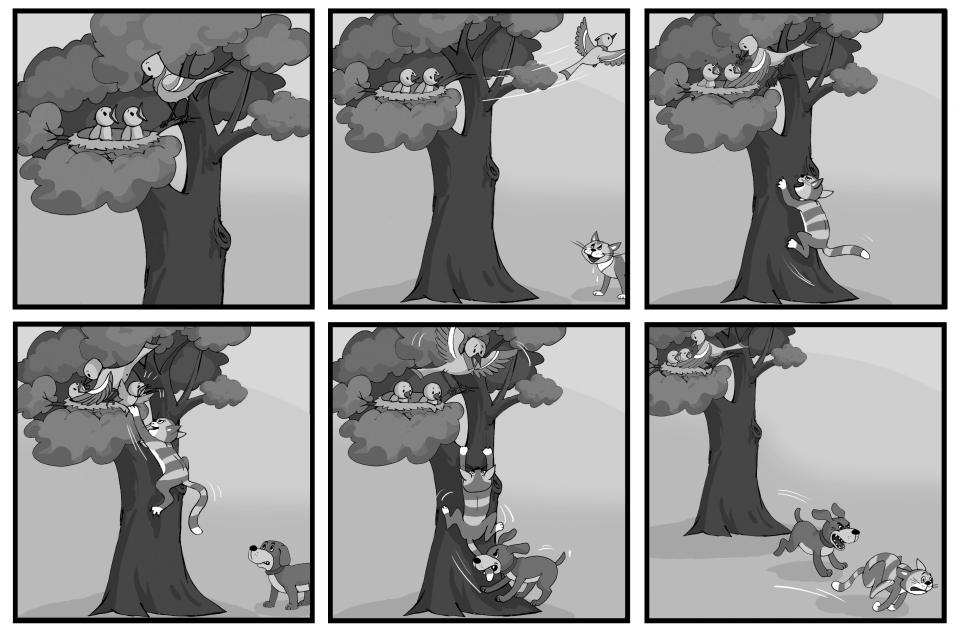
\includegraphics[width=\textwidth]{figures/Chapter6-img001.png}
%   \caption{The Bird story \citep{COST2012}}
% \end{figure}


\subsection{Procedure}

Teams of 3 trainees were formed and instructed to find a 3 to 4-year-old child from a family (usually from their own family and friends, local environment, or members of university staff) who were interested and agreed to let them carry out a study on the child’s linguistic background and linguistic skills in Basque and Spanish. The preliminary data were first presented by each group in English on posters showing the uniqueness of each child’s linguistic background with regards to sociolinguistic context in the Basque Country, family constellation and schooling.

One of the students introduced him/herself to the child as Basque-speaking, one as Spanish-speaking and one as bilingual. This was in order to apply the "one-person one-language" principle when using the Peabody test and eliciting the Bird story narration. The parents were asked to complete the questionnaires in both Basque KGNZ III and Spanish (translated KGNZ III).This ensured that at least one of the parents was a proficient Basque speaker.

Furthermore, trainees were asked to write a report reflecting in English on the language acquisition process, on the child’s anxiety and strategies in encounters with a new language and on the age appropriate teacher intervention for language development. These reports were also presented orally in English in front of classmates.


\begin{figure}
  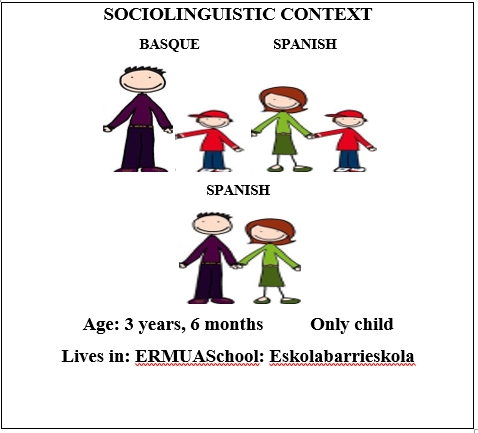
\includegraphics[width=.5\textwidth]{figures/Chapter6-img002-Edited.jpg}
  \caption{Example of a student group poster}
\end{figure}
% \todo{Need better resolution}


\subsection{Findings}
\subsubsection{Children’s data}

As reflected in \tabref{tab:6:1}, data on 20 children, aged from 2:07 to 4:01, were collected by the same number of student teams. These teams were formed of 3 students. The average age of the children was 3:07 and there were 12 girls and 8 boys. Most data were collected in the Mondragon region, which is fairly Basque-speaking, so young children were expected to be Basque-dominant. Based on data on the amount of input in both language as reported on the KGNZ questionnaire by parents it was possible to appreciate whether the child was Basque dominant, Spanish dominant, or had balanced input, or input from another language.

\begin{table}
\begin{tabularx}{.8\textwidth}{Xr}
\lsptoprule
Language & Nº of teams\slash children\\\midrule
Basque dominant & 13\\ 
Spanish dominant & 4\\
Balanced & 3\\
English & 1\\
Wolof & 1\\\midrule
Total & 20\\\lspbottomrule
\end{tabularx}
\caption{Nº of subjects and linguistic characteristics\label{tab:6:1}}
\end{table}

It is also worth noting that many parents who are L2 speakers of Basque tend to make an effort to speak Basque with young children, before language use becomes more complicated and they tend to speak less Basque when demands on parental language skills grow.

From \tabref{tab:6:2} it can be concluded that most children had developed both Basque and Spanish to a level that made it possible to measure language skills with the instruments selected, except in relation to the Bird story in Spanish. Only 10 children out of 20 had attained sufficient expressive vocabulary to be able to produce coherent utterances in Spanish.

\begin{table}
\begin{tabularx}{.8\textwidth}{Xr}
\lsptoprule
Bird Basque & 18\\
Bird Spanish & 10\\
Peabody Basque & 19\\
Peabody Spanish & 18\\
CDI Basque & 19\\
CDI Spanish & 18\\\lspbottomrule
\end{tabularx}
\caption{Tests collected by students\label{tab:6:2}}
\end{table}


\subsubsection{Student presentations}

Having collected the data and completed a guided written report of it, each group of students presented the results of their OCLP project orally, in English, before the class. The aim was to make students aware of the diversity of linguistic microcosms that could be found in children within the age-groups they would be likely to be teaching in their future careers. The presentations were not recorded because this cohort expressed that they would not feel comfortable before the camera, but this could be done in future studies.

Through the presentations, it became evident that 3 languages constitute these students’ DLC \citep{Aronin2016}. They all switched fairly freely between Basque and Spanish when commenting among themselves on how to proceed and it is difficult to know whether they are dominant in one language or the other. However, they took care to express themselves in English when facing the audience, aware that this was the language of the classroom context. They had no special difficulties in oral expression in English, which was sufficiently fluent and only needed occasional support by written texts. Their presentations were easy to follow and well structured.

As to recurring comments in the presentations, many of them expressed their initial frustration in relation to the gap between the results of the Bird story and the Peabody test, until they had realised that they were dealing with the difference between production and comprehension. This was found to be especially striking in Spanish; all groups confessed they had thought most children did not know any Spanish until they discovered that Peabody comprehension scores were higher than expected in Spanish.

Other interesting comments were made on lexical incorporations from one language to the other and some examples were given: \textit{de compras} (`shopping'), \textit{morditu} (`morder' in Spanish; `bite') in Basque by a Spanish dominant child, \textit{eztetnai} (`I don’t want to') in Spanish by a Basque dominant child. Through working with the KGNZ parental report questionnaires they discovered that there is a common, conceptual vocabulary which is reproduced in both languages – although not always: “they know the same words in different languages but some only in one language – and not necessarily the first language”.

All the students pointed out that they had evidenced a high influence of family and environment on the children’s linguistic development, and stressed the importance for future teachers to have knowledge of different types of sociolinguistic situations, as well as of language acquisition in a bilingual community. Their reflections on their own language learning in English and appreciation of having been able to apply theoretical knowledge acquired were very gratifying to the tutors involved.  


\subsubsection{Students’ written reflections}


An analysis of the discussion and conclusion sections of the guided reports submitted by the trainees provides insights into their meta-linguistic awareness, attitudes and emotions in addition to their English language proficiency. In the following, we will present some examples of the most representative aspects from the students’ written reports. The extracts are reproduced in the students' own words, to reflect the general standard of their written English production. These reports have been taken from work submitted electronically for assessment, and the students may have used dictionaries or other electronic support when preparing them. Individual hand-written reports were also made under exam conditions and are the subject of a further study.


\subsubsubsection{Dealing with tensions}


In the first place, there was a general positive feeling about working in a team, sharing knowledge and experiences. Working in teams of 3 is stressed by the students as a very positive factor that greatly contributed to the good results:

\begin{quote}
 In our group we have worked very hard to carry out this project. In most times we have worked separating the work and helping each other, in the doubts we have had.
\end{quote}

\begin{quote}
Despite we have some difficulties we have had some greatest satisfactions about our work in the project. We are proud because we have been able to carry out the project. It has been possible because we have had a really good communication and confidence in the group. So, group work has been great and we have organized what we had to do. 
\end{quote}

The students were instructed to meet the children and their families, whenever possible, on two different days, in order to separate languages and apply the “one person – one language” principle. However, it proved difficult to find family availability for more than one day of tests. In about half the cases both languages were used on the same day, as explained in the following:

\begin{quote}
At the beginning, our idea was to meet with N. two times, on the 20\textsuperscript{th} of March and on the 8\textsuperscript{th} of April. But one day before, N’s mother called us to say that she couldn’t meet with us. That way, the only day that we could meet with N, was on the 8\textsuperscript{th} of April.
\end{quote}

Most groups confess that at the start, they felt uncertain about how to approach the children and about how to handle the tests. The students describe their own feelings about the different sections of the project, the difficulties they encountered and how they gained confidence. They also interpret the child’s feelings: shy, relaxed, comfortable, wanted to play, bored:

\begin{quote}
She did not tell us anything because she did not want and the level of Spanish she has was not very good so she was a little bit embarrassed.
\end{quote}

\begin{quote}
The first day we did the exercises in Spanish and she was very shy. After we did the Peabody test and we showed her the pictures and explain her what she had to name them she was more relax... 
\end{quote}

\begin{quote}
The child respond to the activities but he is very small and he wanted to play with his toys.
\end{quote}

The initial frustration when the children did not respond to some of the tasks was replaced by the insight that with children, flexibility is needed and the best-laid plans may not be possible to carry out. Time must be limited and activities should not be imposed:

\begin{quote}
When we finished with the story, N. told us that she was very bored and tired. That way, we changed the plan that we had at the beginning and we had lunch with them to continue.
\end{quote}

\begin{quote}
When we give her the bird story, she started to opened and closing, turning around... but she wasn’t interested to told us the story. So we decided to not forced her and we let her doing what she wanted.
\end{quote}

When discussing the results with the students it was reiterated that the aim of this study was not to produce a definitive, and scientific, picture but rather an overall impression of one child and their linguistic context. It was made clear to the second year undergraduate students that usually, in order to carry out such tests rigorously, laboratory-like conditions, specific training, and examination of validity and reliability would be required but this was not the objective for the project.

\subsubsubsection{Knowledge gained during the process}


There was a general positive feeling among the students towards the ability they gained as to the use of the instruments and they really enjoyed dealing with the data, making lists, comparing MLUm, MLUw and the Peabody profiles:

\begin{quote}
The biggest difficulty we have had with this project has been the part in which we had to count the morphemes of the longest sentences in the bird’s story and those of MacArthur. We had to ask for help for this and after the explanation it has still been difficult for us, but when we finished it we felt great satisfaction.
\end{quote}

\begin{quote}
J doesn’t say any sentences in Spanish and then we analyze the morphemes of Basque sentences. In the Bird story the sentences are longer than in the MacArthur CDI but the morphemes she used are more or less the same long. We can see the similarities in the MLU since in both of them the results are almost the same.
\end{quote}

All reports reflected that students had realised that the amount of input in the languages the child is exposed to has a decisive influence on its linguistic development. The variety among children also became significantly clear:

\begin{quote}
During the project can be seen very well that L’s language is reflected in her linguistic background. She knows better Basque than Spanish as many people of Azkoitia. As \citet{Palenham2004} says, all normal children brought up in a normal social environment acquire the language of that environment.
\end{quote}

Finally, their theoretical studies on language acquisition could be put into practice and all of them stressed the importance of this experience for them as future teachers:

\begin{quote}
Throughout this project we have learned many interesting things about different languages acquisition. We have read lots of articles to have enough theory before analyzing H’s linguistic development. We have to say that it has been very interesting to apply all the theory in reality, analyzing the real linguistic evolution and situation of the child.  
\end{quote}

As previously discussed in relation to the oral presentations, an important discovery for students was the difference between comprehension and production. Students would insist initially that their child “only knows Basque” and took some time for the students to assimilate that their own data revealed that many of the children were able to understand some Spanish although they showed no production.

\subsubsubsection{Students’ meta-linguistic awareness and confidence in their own linguistic preparation}


An analysis of the writing submitted by the trainees throughout the module and at its conclusion provides a wealth of insights into their meta-linguistic awareness, attitudes and emotions and their English language proficiency.

\begin{quote}
To conclude, I have to say that it has been very interesting this module because I have never thought about how I felt or how I learned the second language (Basque) or the foreign language (English).
\end{quote}

\begin{quote}
In the other side the greatest satisfaction in carrying out this project, has been a personal satisfaction; when we have felt that we were able to make and develop a project in English. Apart from that, it has been very satisfactory understand better how a child acquired a second language, and identify the difference between the first and the second language knowledge.
\end{quote}

\subsubsubsection{Attitudes towards teaching}


Many of the students commented on how the contact with the children through the project made them aware of important age-appropriate teacher intervention strategies, language strategies and other strategies they will need to develop in their future as teachers of young children: 

\begin{quote}
To sumarised, to achieve good language learning and a good language development, is important to know the children every day and work with their parents coherently. What is more, the teacher has to take in to account different strategies such as:

\begin{itemize}
\item Speak in whole sentenses
\item Established day care routines
\item Permit to children listen the adult conversations
\item Use the vocabulary that are used everyday
\end{itemize}
\end{quote}

Such features as child anxiety and the need of an appropriate approach by the teacher were also frequently included in the reports:

\begin{quote}
Another thing I have learned is that when teaching a second language you have to be very careful because of the language anxiety. For that reason, the teacher he/she has to spoke clearly, made eye contact, made feel confortable. In one future I am going to be a teacher so I think this kind of thing can be important to help to children in the learning language process.
\end{quote}

 \section{Conclusions}


We perceive that a number of conclusions can be drawn from the tasks carried out during our project. In the first place, the trainee teachers’ linguistic repertoire comprising Basque, Spanish and English permits them to make an instrumental use of all three languages for educational purposes. Although it was already clear that their level of Basque and Spanish was high enough for the studies they are currently involved in, the present work also shows that they have been able to present their oral reports in fairly fluent English (L3) in a natural way, without reading out the texts. Their written reports are complete, well structured and show a sufficient command of the language for the purpose it was designed for. This fact fits well with the “multi-competence” perspective expressed by \citet{Aronin2016}, since the aim of the task was not to evaluate native-like competence but to make students feel their L3 can serve as a tool for gaining and presenting knowledge acquired. In this sense, students’ reports reflect the confidence gained in relation to their L3 skills and the realisation that English indeed forms part of their dominant language constellation.

In second place, they also reflect the satisfaction felt when realising they are able to handle the instruments used for evaluating language development, by interpreting the children’s feelings and reactions and by overcoming their own uncertainty. In this context it should be born in mind that children’s data should be interpreted with caution. On the one hand, students, although acquainted with tools for data collection, are not yet scientifically schooled enough to make these data reliable, and on the other, all the tools used had not been standardised for scientific purposes.

In third place, students seemed to appreciate the value ofthe knowledge of child language that they had acquired by carrying out the OCLP project for them as future teachers, particularly as two (or more) languages are involved.These results corroborate the importance of specific teacher training in bilingual contexts.  Last but not least, students also referred to their new awareness of the complexity of family life, experienced first hand when fitting their OCLP visits around children's timetables, illnesses and parental commitments. These are valuable insights for any young teacher.  


\section*{Abbreviations}
\label{sec:abbreviations}

\begin{tabular}{@{}ll}
BAC & Basque Autonomous Community\\
DLC & Dominant language constellation\\
OCLP & One child's linguistic picture\\
\\
\end{tabular}
\begin{tabularx}{.45\textwidth}{lX}
CDI & MacArthur-Bates communicative development inventory\\
MLU & Mean length of utterance\\
\end{tabularx}



\sloppy\printbibliography[heading=subbibliography,notkeyword=this]
\end{document}
